\documentclass[12pt, letterpaper,titlepage]{article}
\usepackage[margin=1.25in]{geometry}
\setlength\parindent{25pt}
\linespread{1.6}
\usepackage[utf8]{inputenc}
\usepackage{amsmath}
\usepackage{amsfonts}
\usepackage{amssymb}
\usepackage{graphicx}
\author{Jacob Bruner}
\title{Personal Project}
% add date 
% add word count
\begin{document}
%\maketitle
\begin{titlepage}
	\centering
\vspace*{.8cm}
     {\scshape\LARGE Dwight School \par}
     \vspace{1cm}
     
     {\scshape\Large Personal Project Report\par}
     \vspace{1.5cm}
     
	{\huge\bfseries The Effect of Music on Emotion\par}
     \vspace{2cm}
	{\LARGE\itshape Jacob Bruner\par}
	\vfill
	{\large Advisor: Ms.~Halle \textsc{Bauer}\par}
	\vfill
	% Bottom of the page
	{\large February 8, 2021\par}

	{\large Word Count: 3493\par}

\end{titlepage}


\tableofcontents
\pagebreak
%-----------------------%

\section{Investigating}
\subsection{Goal,  Global Context,  Personal Interest}
\paragraph{}
My goal was to compose three musical compositions evoking three different emotions and to accompany them with detailed descriptions of their musical devices contributing to emotion.  This goal forces me to demonstrate understanding with how and why musical devices can evoke emotion. By creating three pieces evoking different emotions, I am conveying fluency in emotional storytelling. I achieved this by using my talents on the piano to create recordings of three different composed piano pieces. Piano is one of my passions; I have been playing the piano since about the age of six. From a young age, my love for the instrument lay in the creative possibilities. I chose this goal because I often don’t get the ability to express myself through music in my standard curriculum. By choosing a personal project I am passionate about, I hoped to enjoy the hard work more. Despite my experience with composition, this goal is still \textit{highly challenging} for me to complete. In more depth, this goal requires me to explore my musical understanding by researching why a given device can evoke emotion. This goal also requires me to articulate my choices in more depth than "It sounded good, so I added it," which will expand my thinking and push my limits as a creative composer. In essence, this goal is challenging because it demands I formalize my creativity and convey my understanding.


\paragraph{}
My global context is Personal and Cultural Expression. It explores human expression and inquires into the methods of expressing ideas, emotions, beliefs, and values. More concisely, it explores human creativity. I believe to a great extent this global context fits my goal and topic of my project because I was exploring a quintessential method of expression: music. I was exploring how music conveys ideas and emotions: a precise value of the global context.  I firmly hold that music is the most effective medium of personal and cultural expression because its ability to evoke emotion is unmatched; therefore, this global context is perfect.



\subsection{Prior Learning}
\paragraph{}
After years of being miserable during piano lessons, I quit. I taught myself the piano of my own accord for about seven years, during which I developed a passion for composition. Within lessons, I could not bear to play exactly what was on the sheet music. The piano teachers mistook my disinterest as inability, resulting in them selecting uninteresting pieces to learn. When I quit, I had the freedom to learn the songs I enjoyed and modify elements I disliked. The first few notable pieces I learned during this time were, Let it Go from Frozen, various songs from \textit{Legend of Zelda Ocarina of Time}, and various video game soundtracks. However, within the past two years, I have resumed taking lessons, but with a much more engaging and supportive teacher that supports my creativity. I am classically trained now, and I am learning the works of Ravel and Liszt. Even within these studies, I have the freedom to choose pieces I am engaged with. In addition, I have leveraged online resources to heighten my understanding of music theory and composition. There is a vast collection of educational content on YouTube I have used to my advantage. Some of the topics I find fascinating are modal interchange, tonal modulation, chromaticism, and harmony in general. I frequently test my abilities by improvisation. This music-specific knowledge was consistently highly relevant and applicable to what I sought to produce as a final project because it allowed me to focus my research on expanding my knowledge and creating something instead of learning the basics. I intended to expand this understanding into intuition for how musical devices can evoke emotion. Part of this was accomplished by research; however, I intended to gain some of it from my creative process. The benefit is that I can make my own musical decisions and discoveries. In a highly interpretive art, my toolbox as a musician must be born of creativity. Examples of projects I have composed in the past include from evocative solo piano pieces to down-tempo jazzy ambient songs. The latter of which is a song, tilted ‘Away,’ I published on Spotify. Overall, each of these works contributes to my musical intuition. The musical greats all formed their unique and memorable style through self-discovery and learning, so I believe it is vital to gain insight during this project from my creativity.


\subsection{Research Skills}
\paragraph{}
Throughout this project, I completed a lot of research. The majority of this explored why and how musical devices can evoke emotion, following my research question: “What elements of a musical composition evoke emotion?” Because this is an advanced topic, I found it crucial that my sources and information were high quality, so the vast majority of my sources were from educational institutions. I also sought to include studies and research that credibly drew conclusions; more generally, I looked to find primary sources, including theories directly from the creator. The strengths of these reputable sources are that they were informative and reputable. Much of the information was from college curricula, so the information required a high level of past understanding and the patience to parse through. I also believe the COVID-19 pandemic improved my research ability because these sources were made public following the onset of online learning. One possible limitation of my sources is that they were dense, which means that I had to dedicate time to rereading. One instance of a useful source was a book written by Klaus R. Scherer, published by the Oxford University Press, titled \textit{Music and Emotion: Theory and Research}.  This source provided me much value because it detailed the musical devices that could be used and provided a rich understanding of why something evokes emotion. I completed an OPVL analysis of the notable sources I used (found in the appendix). After researching, I ensured the information I used was paraphrased. I did this by taking detailed notes on each source, then composing without looking at them. The purpose was to ensure I was violating intellectual property and to demonstrate that my finished product was my own understanding. Overall, this research was conducted to assist my understanding of musical devices for my compositions and improve the details of my works’ descriptions.



%-----------------------%
\section{Planning}
\subsection{Criteria}
\begin{figure}[h] 
\begin{center}

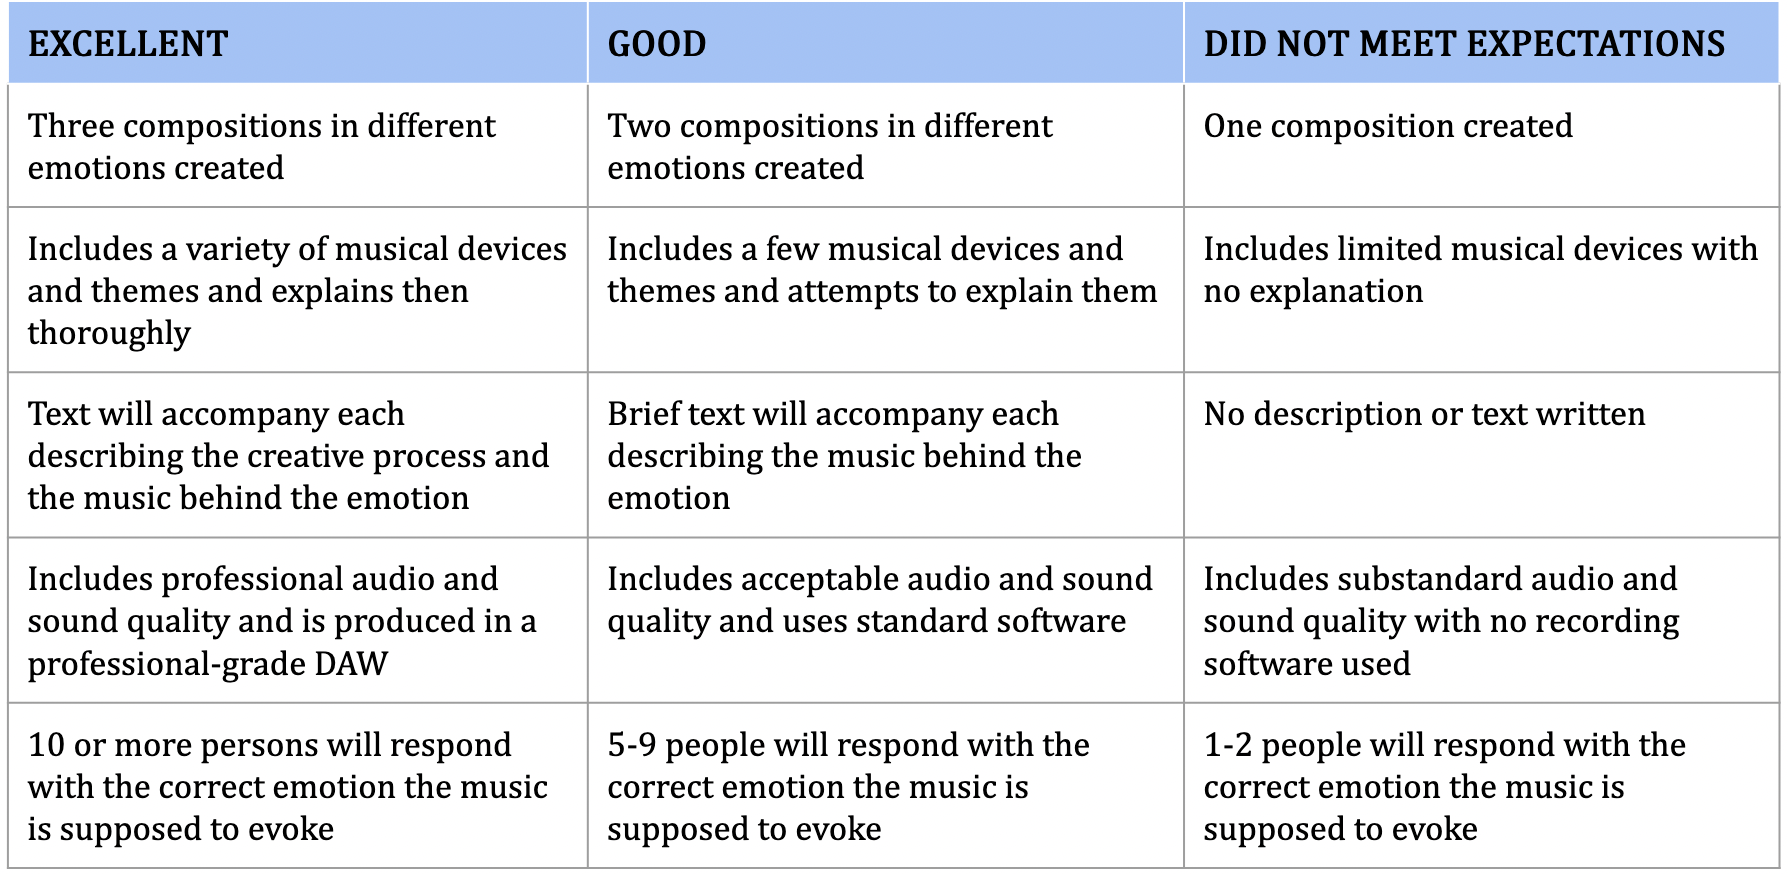
\includegraphics[scale=.53]{rubric}
\caption{Rubric of Criteria}
\end{center}
\end{figure}
\paragraph{}
During my process, I created a rubric of criteria to measure my final product's effectiveness. (Rubric can be found in appendix) I worked hard to ensure these criteria were quantifiable; I wanted to make sure I could measure whether my compositions could evoke emotion. For my project to meet my expectations, I would have to survey people about my music. To achieve excellence, I described that ten people would respond with the correct emotion and agree the composition was effective. Inversely, if nobody surveyed could guess the emotion, then the project would not have met my expectations. Another criterion is that my compositions would contain "a diverse selection," "a few," or "a limited amount" of musical devices. The intention behind this specific wording is because the number of musical devices is not an indication of how effectively they were used. I worded this so it’s not based on a set amount; it will allow me to pursue quality over quantity. Furthermore, to achieve excellence I need to accompany each composition with a detailed written text explaining the devices at play and how they are used to persuade emotion. To achieve excellence, each of my works would include "professional sound and audio quality." This would be accomplished using a Digital Audio Workstation (abbreviated DAW) software and my recording equipment to record a piece. This will be measured qualitatively based on clarity, volume, and sound. To miss excellence, I would produce a song with questionable quality such as noticeable background noise (meets expectations) or a song that is unlistenable and broken up (below expectations). Overall the goal of the rubric is to fairly measure my goal's completion. This rubric is also highly challenging because it required me to push my abilities and create a coherent product.



\subsection{Planning of the Development Process}
\paragraph{}
The personal project is a substantial project requiring a high level of planning to complete thoughtfully. To achieve this, I created a calendar of goals detailing formal due dates for the project and personal due dates to keep my work on track. (This calendar can be found in the appendix.) The calendar demonstrates my willingness to self-manage and mitigate procrastination. I also wanted this calendar to be more accessible, so utilized google calendar. (A recommendation from my Personal Project Advisor.) I did this because it sent notifications to my phone. Therefore, I was able to allocate time to working on this project by making smaller goals day-by-day: making the larger goals digestible. I also used music planning documents to organize my creative process. When writing music, I took detailed notes about how, where and why I used a specific musical device. This planning made explaining my compositions easier because my ideas were already written down. I used these planning documents to speed up the composition process because I did not rely on memorization alone. (Evidence of these music process documents are in the appendix.) Overall, I used several different methods to plan to complete my goal making meeting my goal more achievable.






\subsection{Self-Management}
\paragraph{}
Throughout this project, I exercised and improved my self-management skills. I knew from experience I often leave work until the last minute; therefore, coming into this project, I intended to organize myself such that I would be able to meet deadlines. This led to self-discovery because it required me to practice self-discipline. At the beginning, I had planned my deadlines and my work; however, I struggled with time management. I admit I was unable to complete my first few self deadlines. One example of this was when I completed my rubric of criterion five days after I intended to. However, I had to stay calm and understand there was room for me to improve. From this, I learnt I have to understand delayed gratification and complete assignments promptly. I began using google calendar to allocate chunks of time to working on my project. This proved to be extremely successful as I completed the rest of my work requirements before or by the deadline. One example of this is that I sought to have sections I and II of my written report completed before we returned to school after Thanksgiving. However, I found time and completed these sections three days early. I understood the benefit of completing prior to the due-date when my peers were voicing their complaints about completing the sections on Sunday night, and I could get to bed early. From then on in the project, I met my deadlines and managed my time effectively. Overall, I learnt about managing my own time, and I will apply this information to my other disciplines. Evidence of my self-management techniques can be found in the appendix.


%-----------------------%
\section{Taking Action}
\subsection{Product}
\paragraph{}
As previously mentioned, I intended to meet my goal by creating three musical compositions accompanied by peer feedback and analysis. I selected this challenge because it would help me understand my global context, \textit{personal and cultural expression}, since this project explores how ideas and emotions can be expressed through music. For all three pieces, I began by creatively improvising in the theme of my emotion. I sat down for hours with no goal in mind developing ideas. This process was not without critical thinking, for each move I made during improvisation was a split-second index of my musical vocabulary. Much like speaking a language, I had to string together musical words and devices into coherent sentences and cadences. I did notetaking and early recordings of the ideas I liked. My next step was to try to piece together these ideas and unify them into a single piece. I accomplished this by recording ideas on sheet music, and creating outlines in my notes. Once I felt satisfied with my creation, I dedicated time to producing the song within the software Logic Pro. After the recordings were mixed, I exported the final product. From my musical knowledge combined with my extensive research on the impacts of emotion, I was able to type up informative responses for each piece detailing the music theory behind it and how it was used as a tool to evoke my intended emotion (all three found in project documents). I proceeded to test the effectiveness of my product by performing a blind study in which I surveyed 10 people what emotions they thought the song evoked as well as how effective the songs were at evoking emotion. The participants, my family and peers, did not have a preconceived idea of what I intended. I also established my baseline emotional intent, so I could not retroactively fit the responses of the survey. The survey responses can be found in the appendix. The outcome of this creative process was three unique pieces written for the piano. My first piece is a delicate modal exploration into how complex harmonies can express emotions in the realm of hope, nostalgia, and significance but not without the nuance of difficulty and sacrifice. Some devices include a lack of melody, smooth voice leading, ostinato figures, strumming chords, thick layered extensions, suspended chords, plagal cadences, and chromatic mediants. The second piece has a ‘time’ theme and intends to evoke emotion of armageddon, time running out, climax, and action/conflict. The beginning employed a pentatonic falling melody, as well as a rhythmic focal-point: two bars in 4:4 being split into 5 beats and 3 beats respectively. Towards the end, the song employed lots of dominant b9 and diminished chords to create tension. Throughout the piece there are ostinato figures and frequent use of the 9th and 11th scale degrees. By contrast, the third piece explores travesty and hardship through its unique use of dissonance. The piece is played tempo rubato and has an emotionally-driven middle section thrusting the harmony forward and creating momentum. Following the creation of all three pieces, I spent a couple weeks writing thoughtful analysis of the musical devices I used. Here, I described the pieces’ impact on emotion by explaining techniques from my extensive research into music and emotion. I intended the analysis to demonstrate a high level of understanding. (Each song and description can be found in the project documents)

\subsection{Thinking Skills}
\paragraph{}
At the start of my project, my thinking skills with respect to musical composition were solid.My musical background and passion assisted me from the start. I think this is evident through my goal and rubric of criteria, because those demonstrate an understanding of what makes a musical composition ‘good.’ Furthermore, my thinking skills improved massively during researching and creating because I improved my ability to compose. Evidence of this improvement is the contrast between the first second and third compositions. I think there is a trend of linear growth in how good the recordings sound across 1, 2 and 3. In 3 I used higher quality and more complex recording equipment to create a stereo sound , demonstrating my improved thinking skills with respect to audio engineering. Overall, I think to a great extent my thinking skills improved throughout the course of my personal project.
\subsection{Social and Communication Skills}
\paragraph{}
The process of organizing a project of this scale improved my social and communication skills. I am an independent thinker, so coming into this project I was unable to initially handle reaching out for help. Over time, my skills improved: every time I communicated with my advisor and sought help from peers I grew a bit more confident in my ability. I communicated with my advisor, Ms. Bauer, regularly. I scheduled meetings and met to discuss the project. These meetings became more useful as my communication skills improved because I could use the time to ask more specific questions. (Evidence of our meetings can be found within the appendix.) In addition, my social skills improved from obtaining peer feedback. I frequently sought feedback from my music teacher and peers regarding the effectiveness of my musical choices. These interactions helped to improve my social skills because I had to ask for feedback. Towards the end of the process, I displayed my social skills in full form when I reached out to 10 people to evaluate my music. Overall, this project helped me improve my communication skills to a great extent.

%-----------------------%
\section{Reflecting}
\subsection{Evaluating the Product}
\paragraph{}
Following the completion of my compositions, analysis, and peer feedback, I believe I met the criterion of success I outlined. I met the primary goal of my project: to create three distinct musical compositions. In the second category, I argue I met my goal of including a variety of music devices and explaining them thoroughly. My song descriptions reflect detail and research, so I fall under ‘excellent.’ Similarly, I created three descriptive texts for each piece, which puts me under ‘excellent’ for the third criterion. On the fourth criterion, I fall between the ‘excellent’ and ‘good’ categories. My third composition reflects “professional audio quality,” however I think my first and second reflect “acceptable audio quality.” All three were created in Logic Pro X--a professional DAW--though. Lastly, I met my most difficult criterion because all 10 of the surveyed people responded with exactly the emotion I was intending. 
\begin{figure}[h] 
\begin{center}

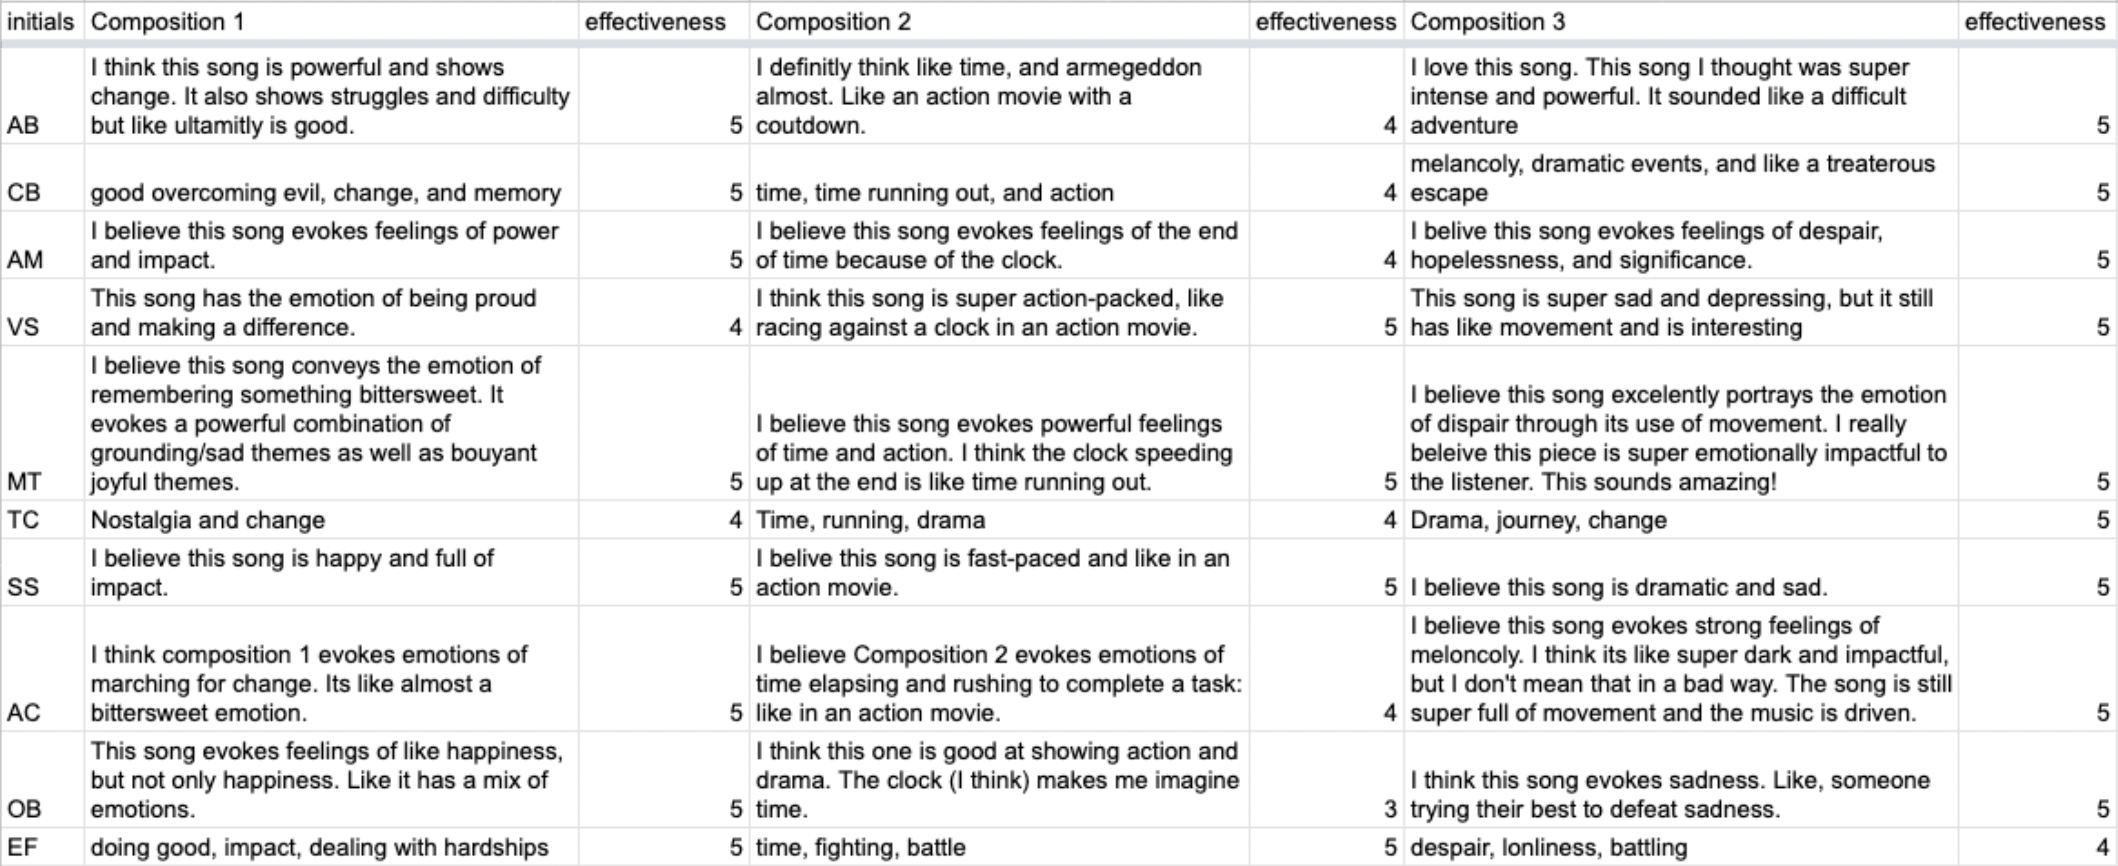
\includegraphics[scale=.4]{survey responses}
\caption{Table of the 10 Survey Responses}
\end{center}
\end{figure}
For compositions 1, 2 and 3, all responses fit under the umbrella of change, running out of time, and hardship respectively. Furthermore the average emotional effectiveness from 1-5 for each was 4.8, 4.3, and 4.9 respectively with a 5 being “extremely effective.” Overall, my final project falls within the realm of ‘excellence.’ The strengths of my outcome were the emotion conveyed in the individual pieces. All three turned out better than I had imagined. Another strength of this product is the growth of my passion. If I were to complete this project again, I would invest more time into producing and mixing the first and second pieces.

\subsection{Understanding the Topic, Global Context, and Myself}
\paragraph{}
During this project, I faced a number of challenges for which I had to adapt to. I faced personal challenges with trying to explore composition techniques I was unaccustomed to. Starting a composition from the emotional perspective instead of from an academic perspective provided me a difficult test of my abilities to adapt to unfamiliar applications of my knowledge. On a more project based scale, I faced the challenge of  budgeting my time. Often I fought against my tendency to procrastinate. I employed tactics to improve my ability to get stuff done. Most notably, this project gave me the opportunity to consolidate my schedule and use a calendar. I used  google calendar to manage my self-imposed due dates as well as set day-to-day reminders and study times (evidence found in appendix). I also learnt how to use a process journal to organize my project; I used a google drive to organise important documents (evidence in appendix). An entry that assisted my project was a halfway self-assessment. I believe my communication skills were improved following this reflection. Overall the ability to manage my time in this way is undoubtedly a skill I will retain and use throughout my life, so I am grateful that this project gave me the opportunity to grow. From a holistic perspective, I believe the product of my personal project reflects a growth in my understanding of not only music, but art and forms of expression. The global context of ‘personal and cultural expression’ gave me insight into how emotion drives expression. My ability to successfully tailor the musical mode of expression to specific emotions conveys my growth in ability to classify and analyse expression through music. 
\subsection{IB Learner Profile}
\paragraph{}
I believe as a result of this project, I improved my IB Learner Profile skills of being a thinker, knowledgeable, a risk-taker, and a communicator to a great extent. I improved my thinking skills by researching and implementing new creative ideas from my research.  I became more knowledgeable about music theory and emotion. I became more of a risk-taker within my creative process, because I tried testing new musical devices to create an emotional atmosphere. Lastly, I improved as a communicator because I had to reach out to my peers and advisor throughout the project. I believe my product was successful, but if I were to do it again, I would have done more research into how to create high-quality recordings of the piano. Additionally I encountered the constant threat of procrastination. I think I tried and had good success in managing my time, but I still believe I could have improved it more. I think this weakness contributed to the level of stress I felt throughout, and made some of the work more difficult especially at the beginning.
\paragraph{}
In summary, I believe the personal project helped me improve critical skills that I will continue to use throughout my life as a learner. I think these skills will assist me in completing the DP program. Most notably, I think my improved ability to organize, time-manage, and communicate will be invaluable for my future; I am grateful that this project gave me the opportunity to improve.


%-----------------------%
\newpage
\section{Appendix}
\subsection*{OPVL Analysis}
\begin{center}
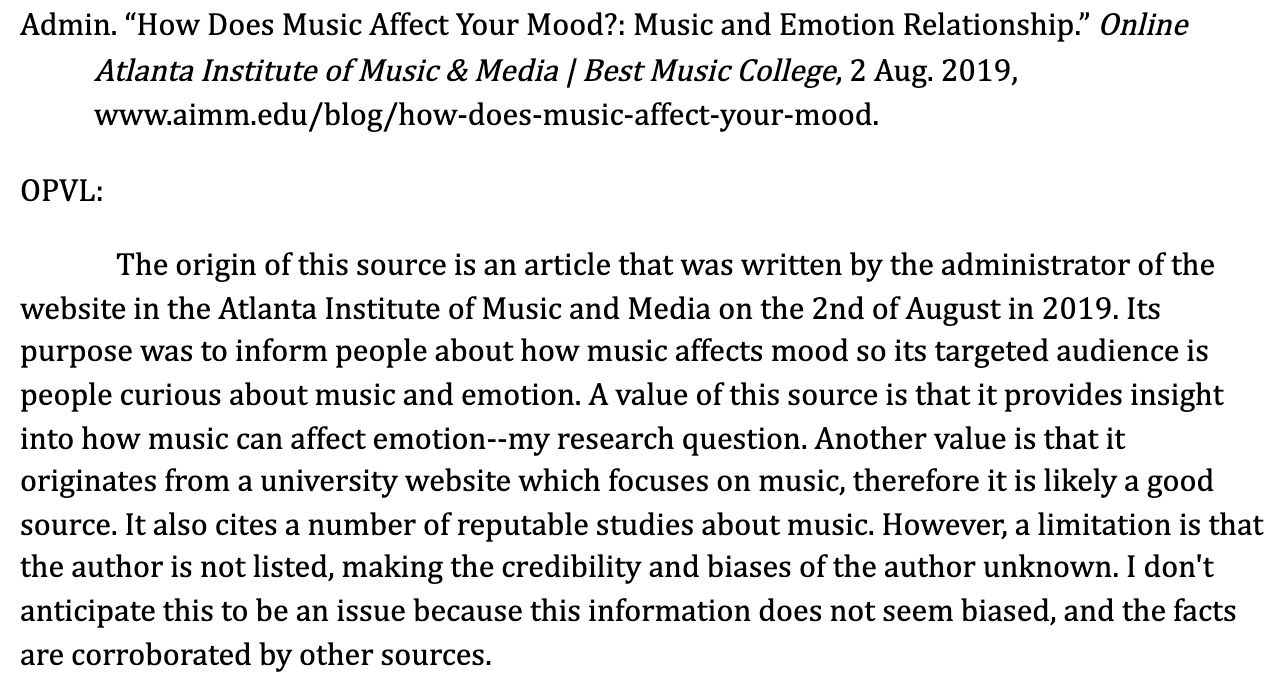
\includegraphics[scale=.65]{1} \\
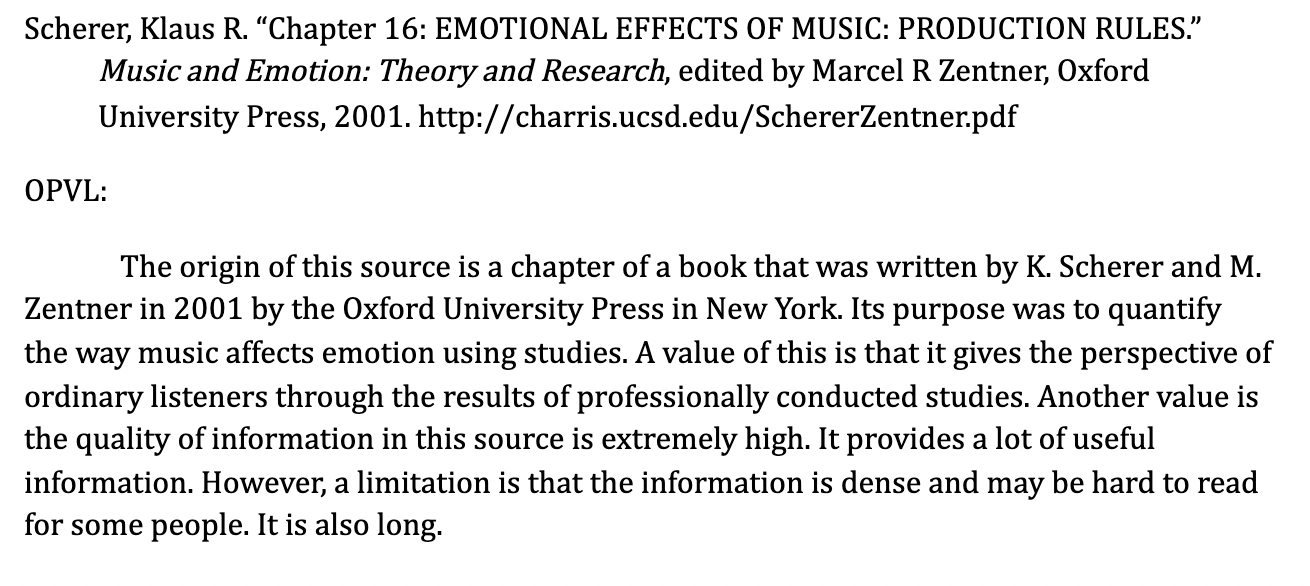
\includegraphics[scale=.65]{2} \\
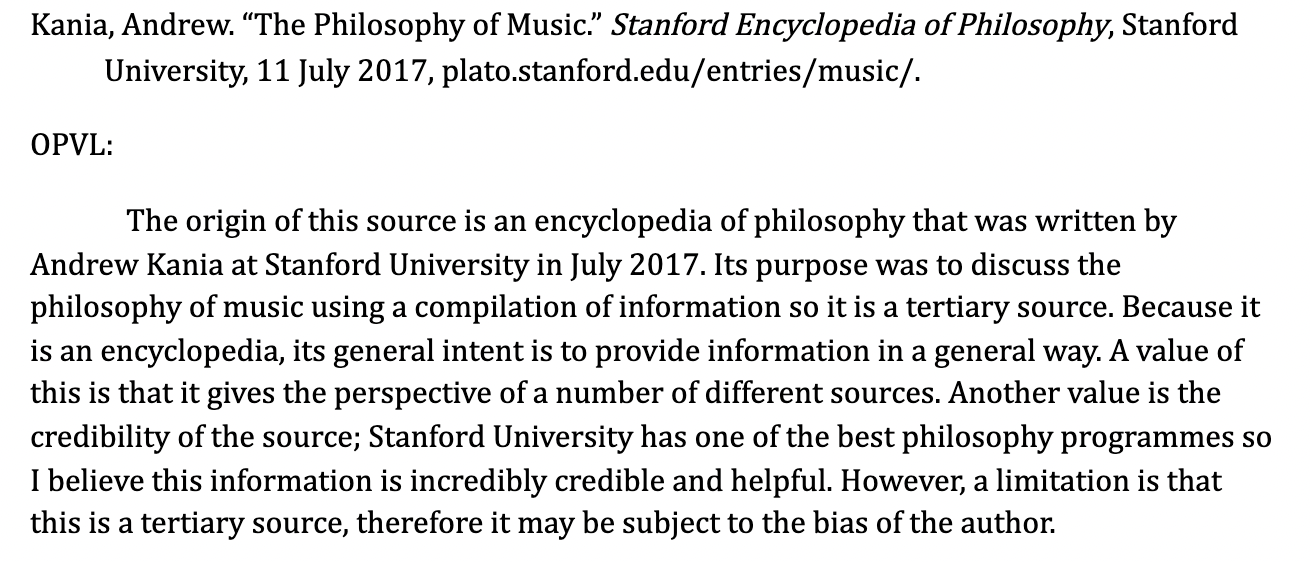
\includegraphics[scale=.65]{3} \\
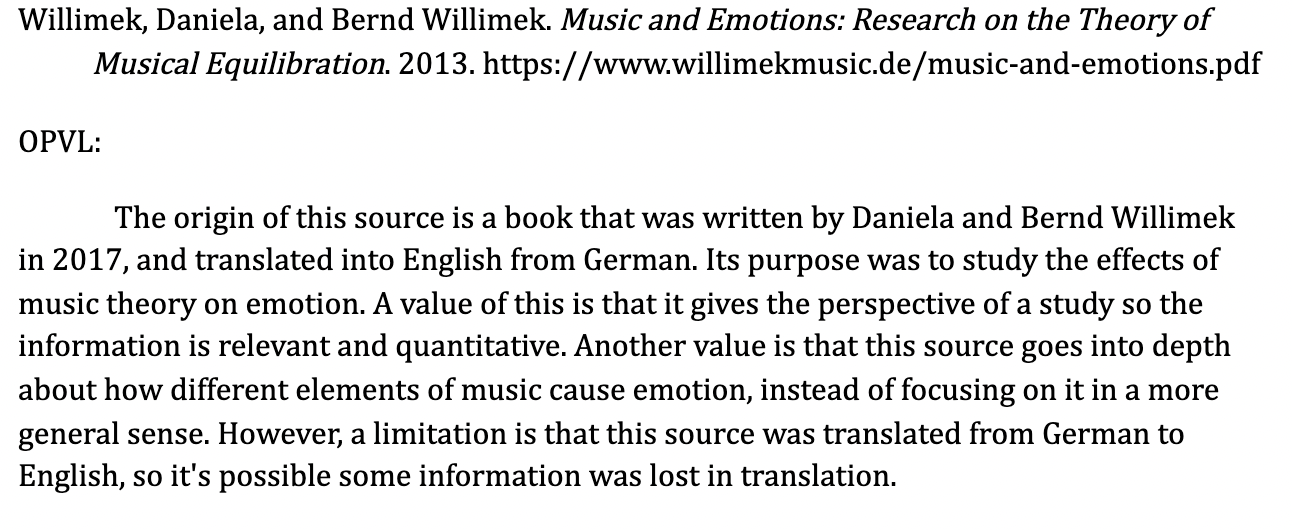
\includegraphics[scale=.65]{4} \\
\end{center}
\newpage
\subsection*{Calender of Deadlines}
\begin{center}

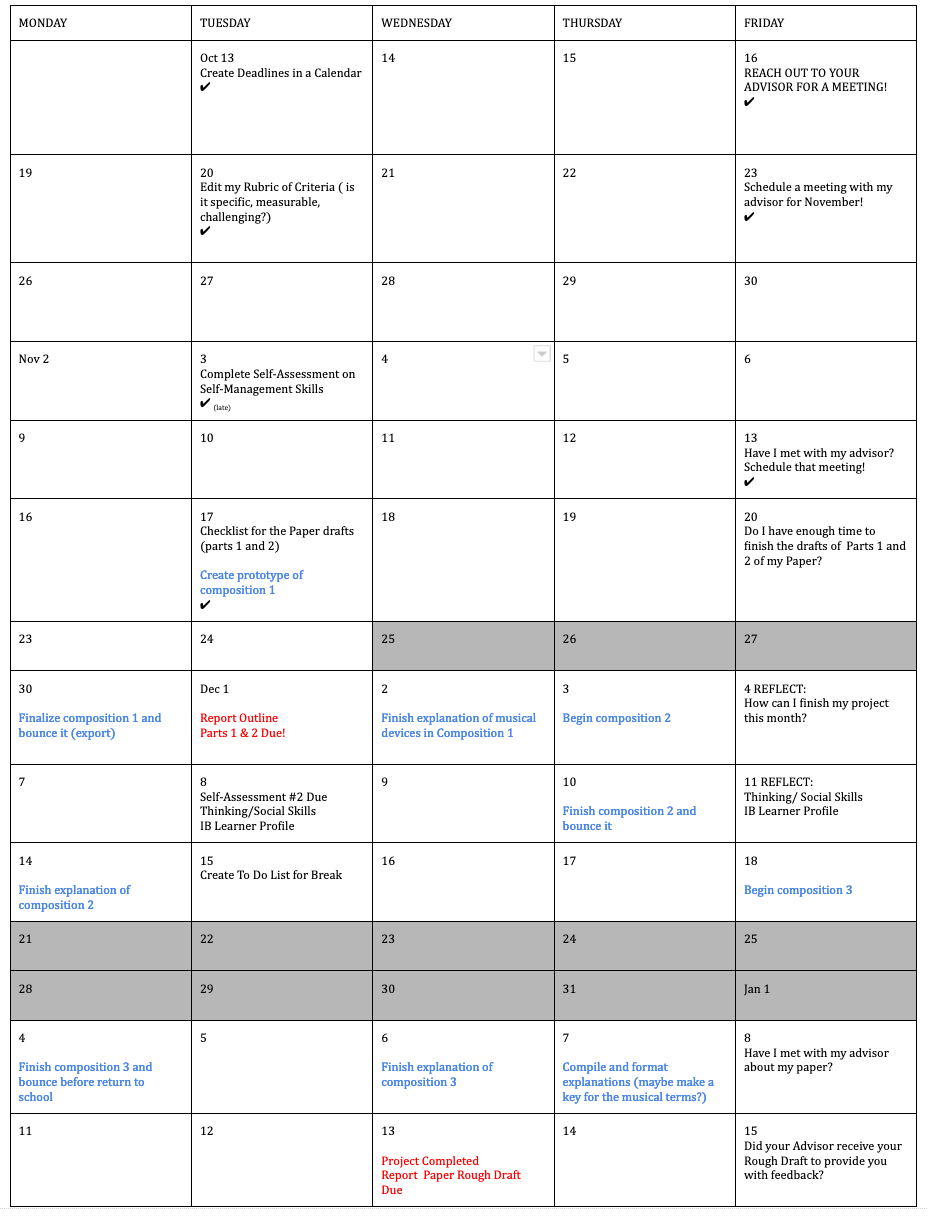
\includegraphics[scale=.95]{calender}
\end{center}
\subsection*{Emails with Advisor}
\begin{center}
\hspace*{-1.2cm}
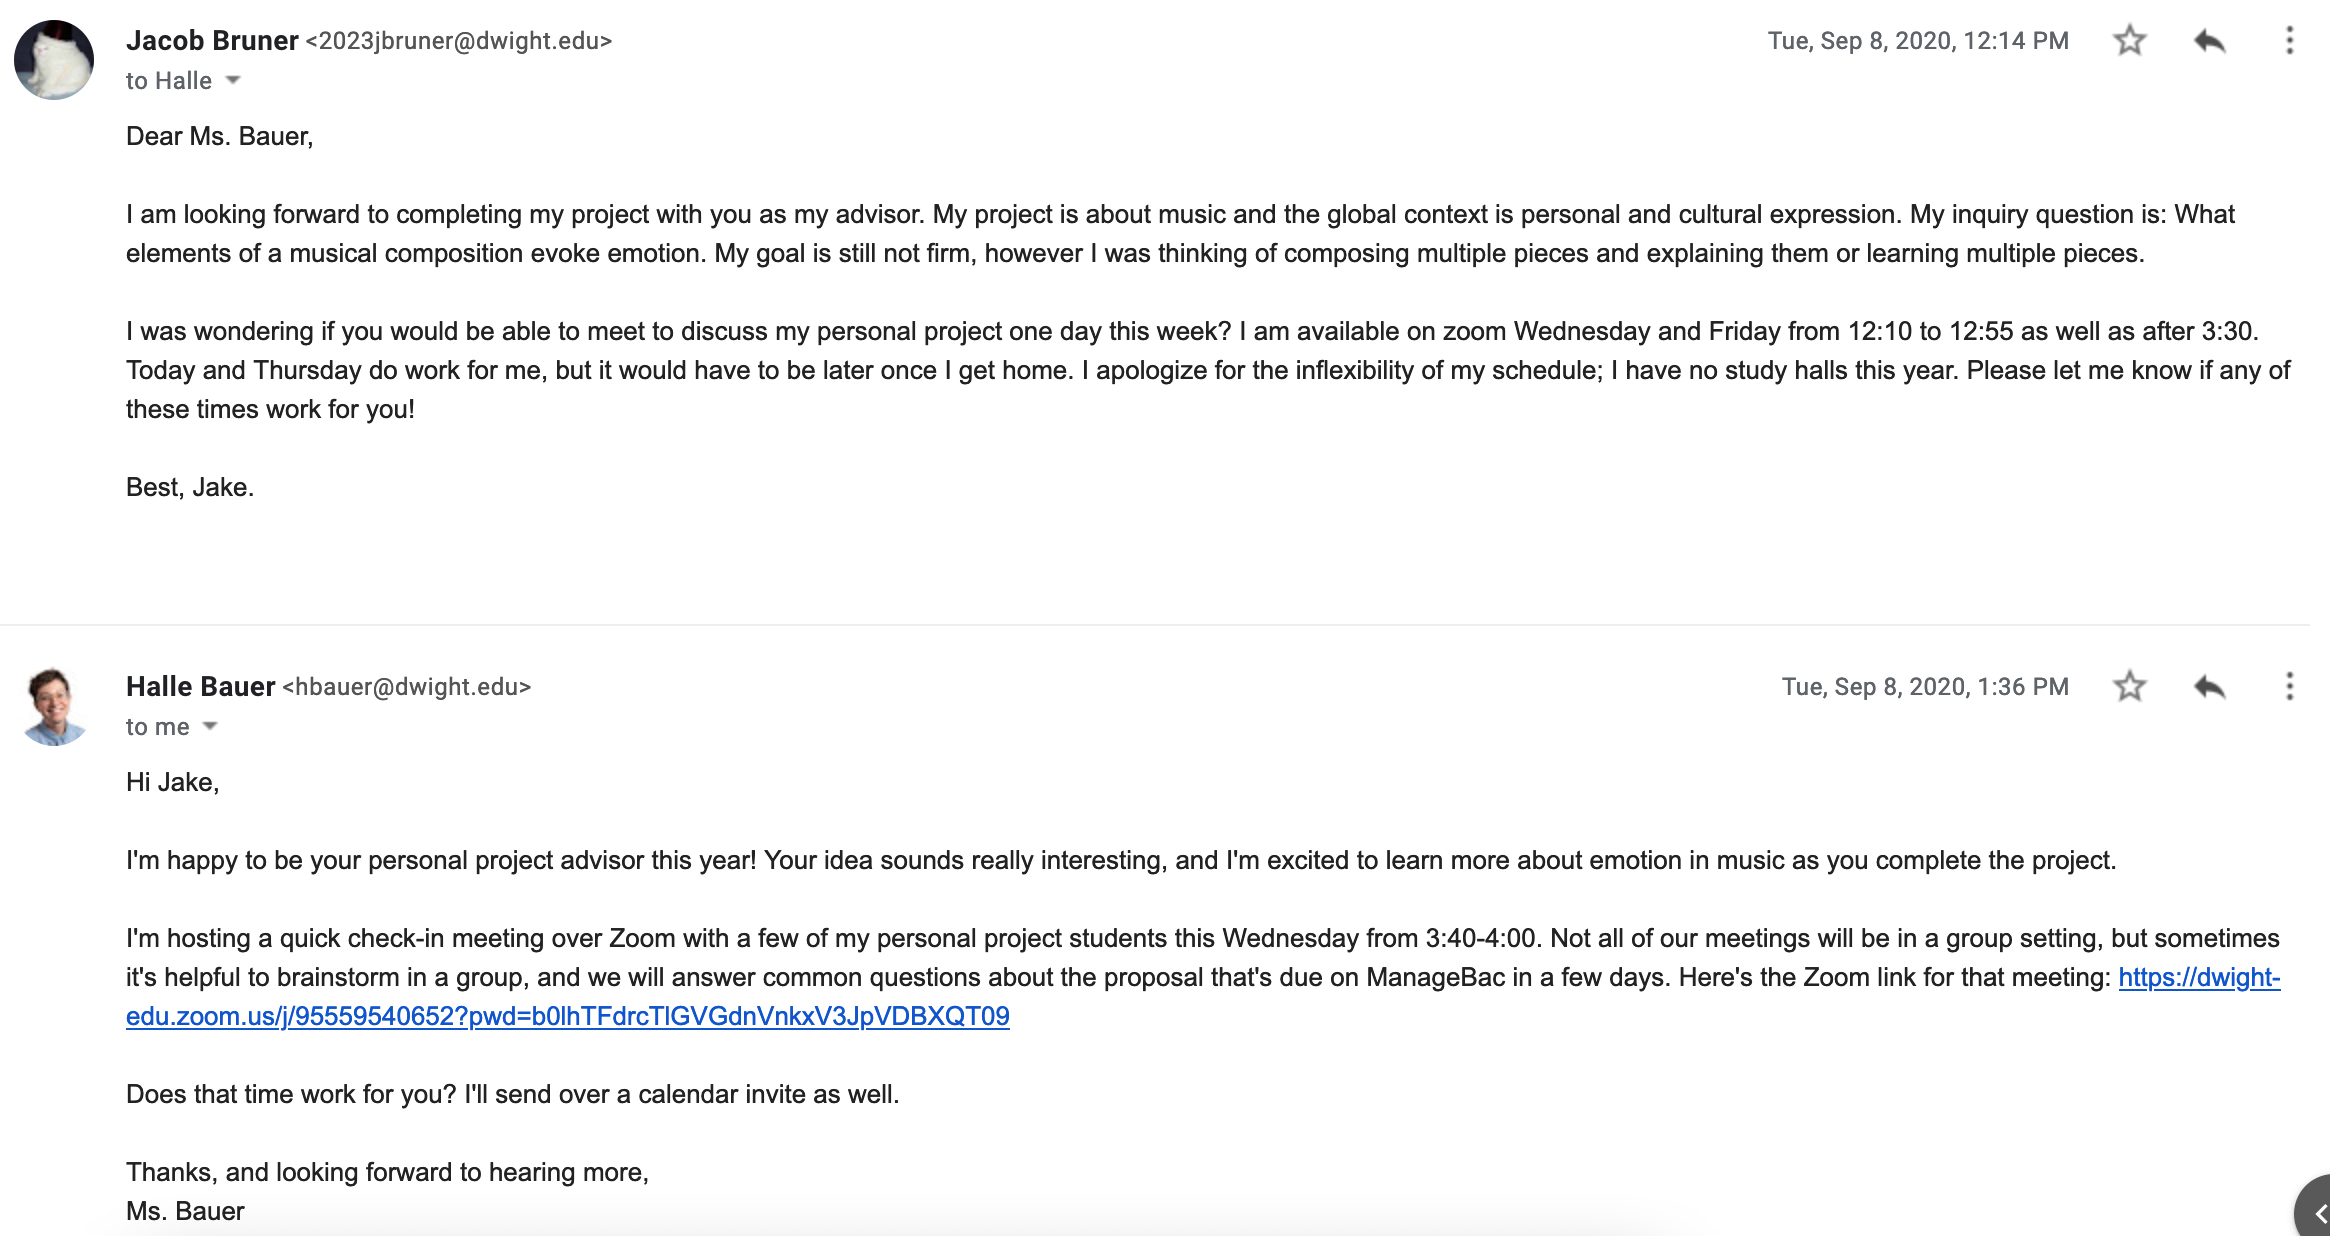
\includegraphics[scale=.43]{email1}
\hspace*{-1.2cm}
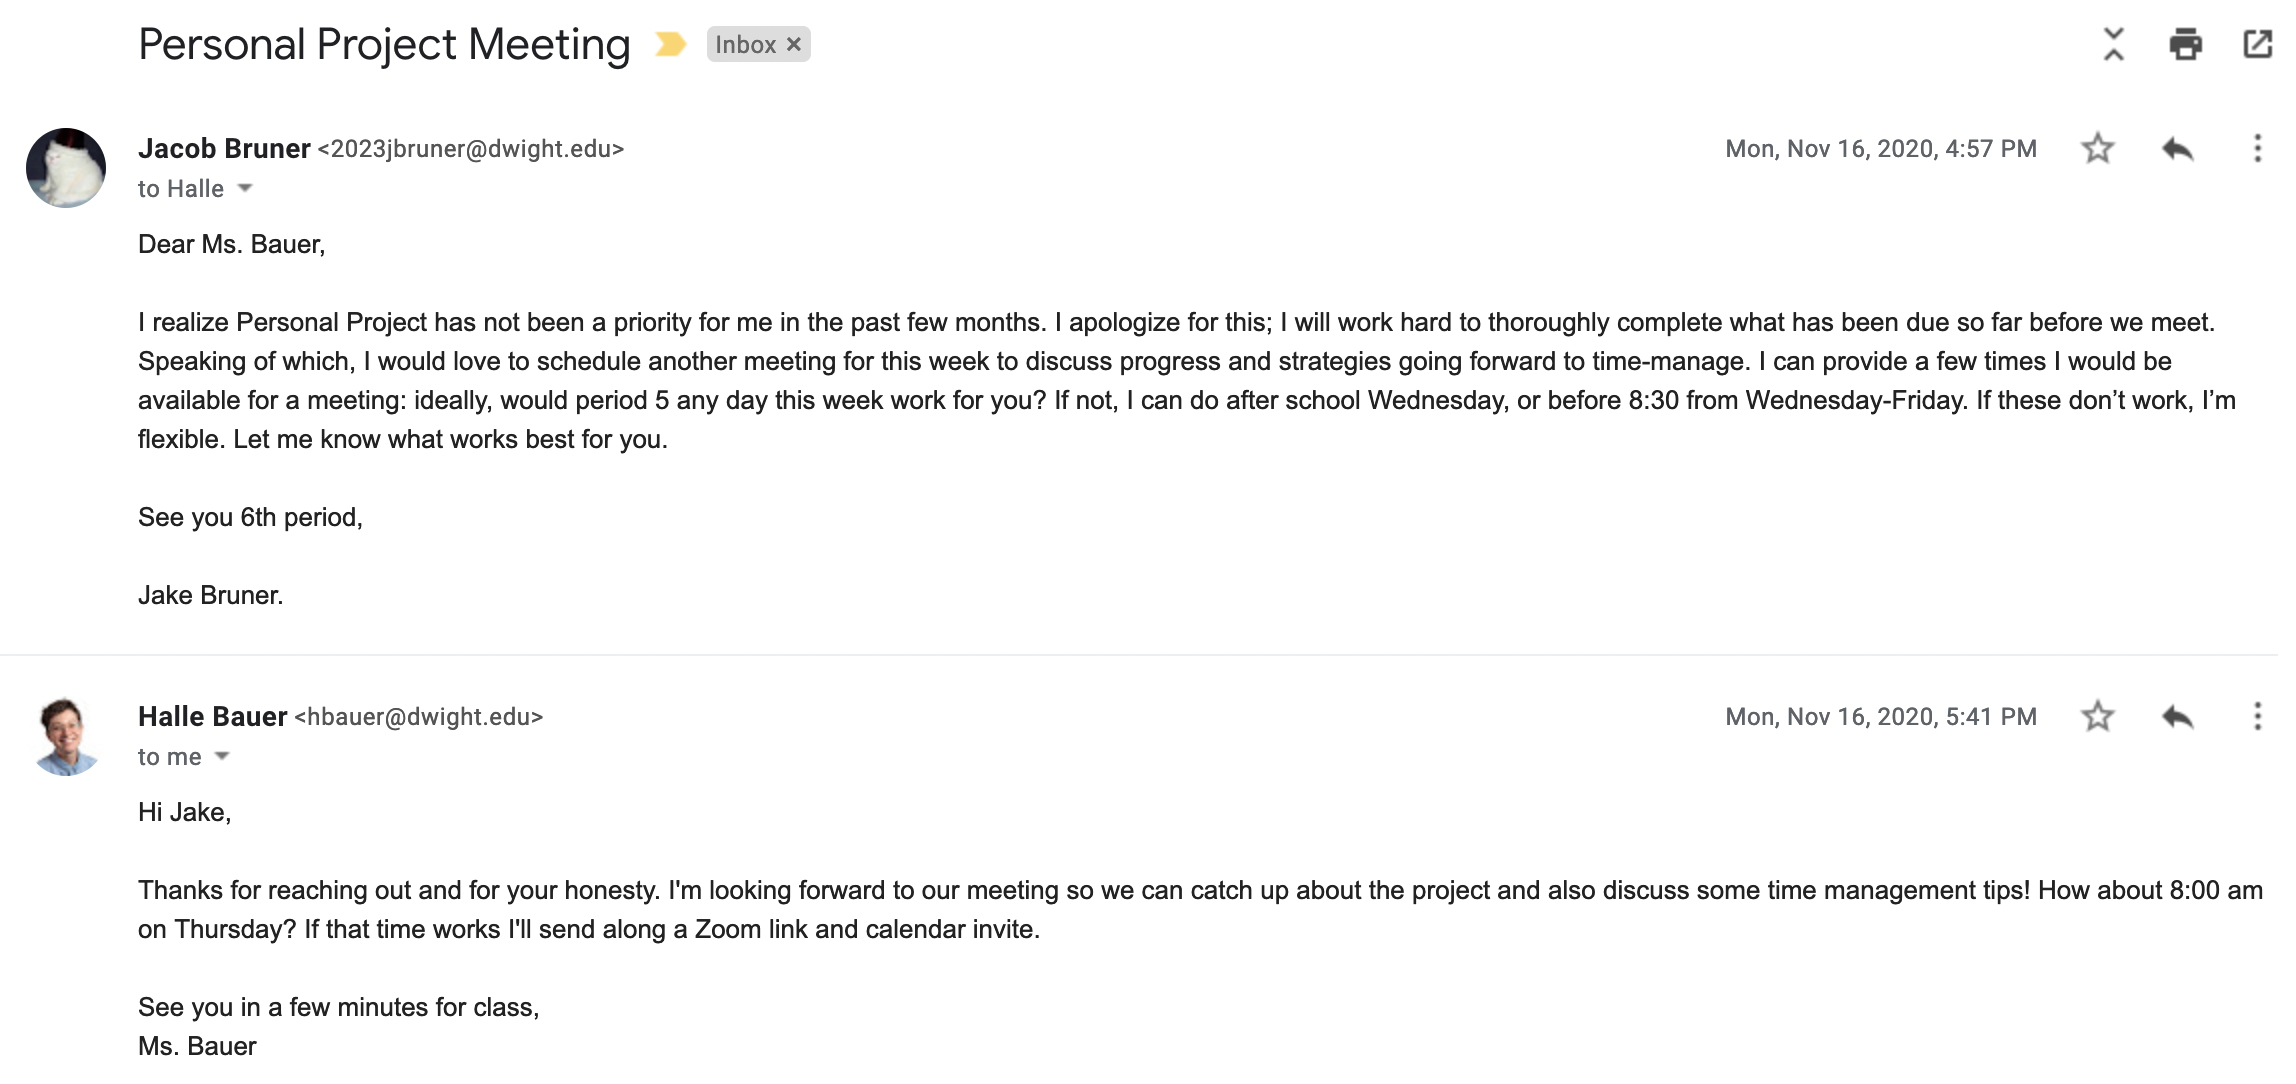
\includegraphics[scale=.43]{email2}
\hspace*{-1.2cm}
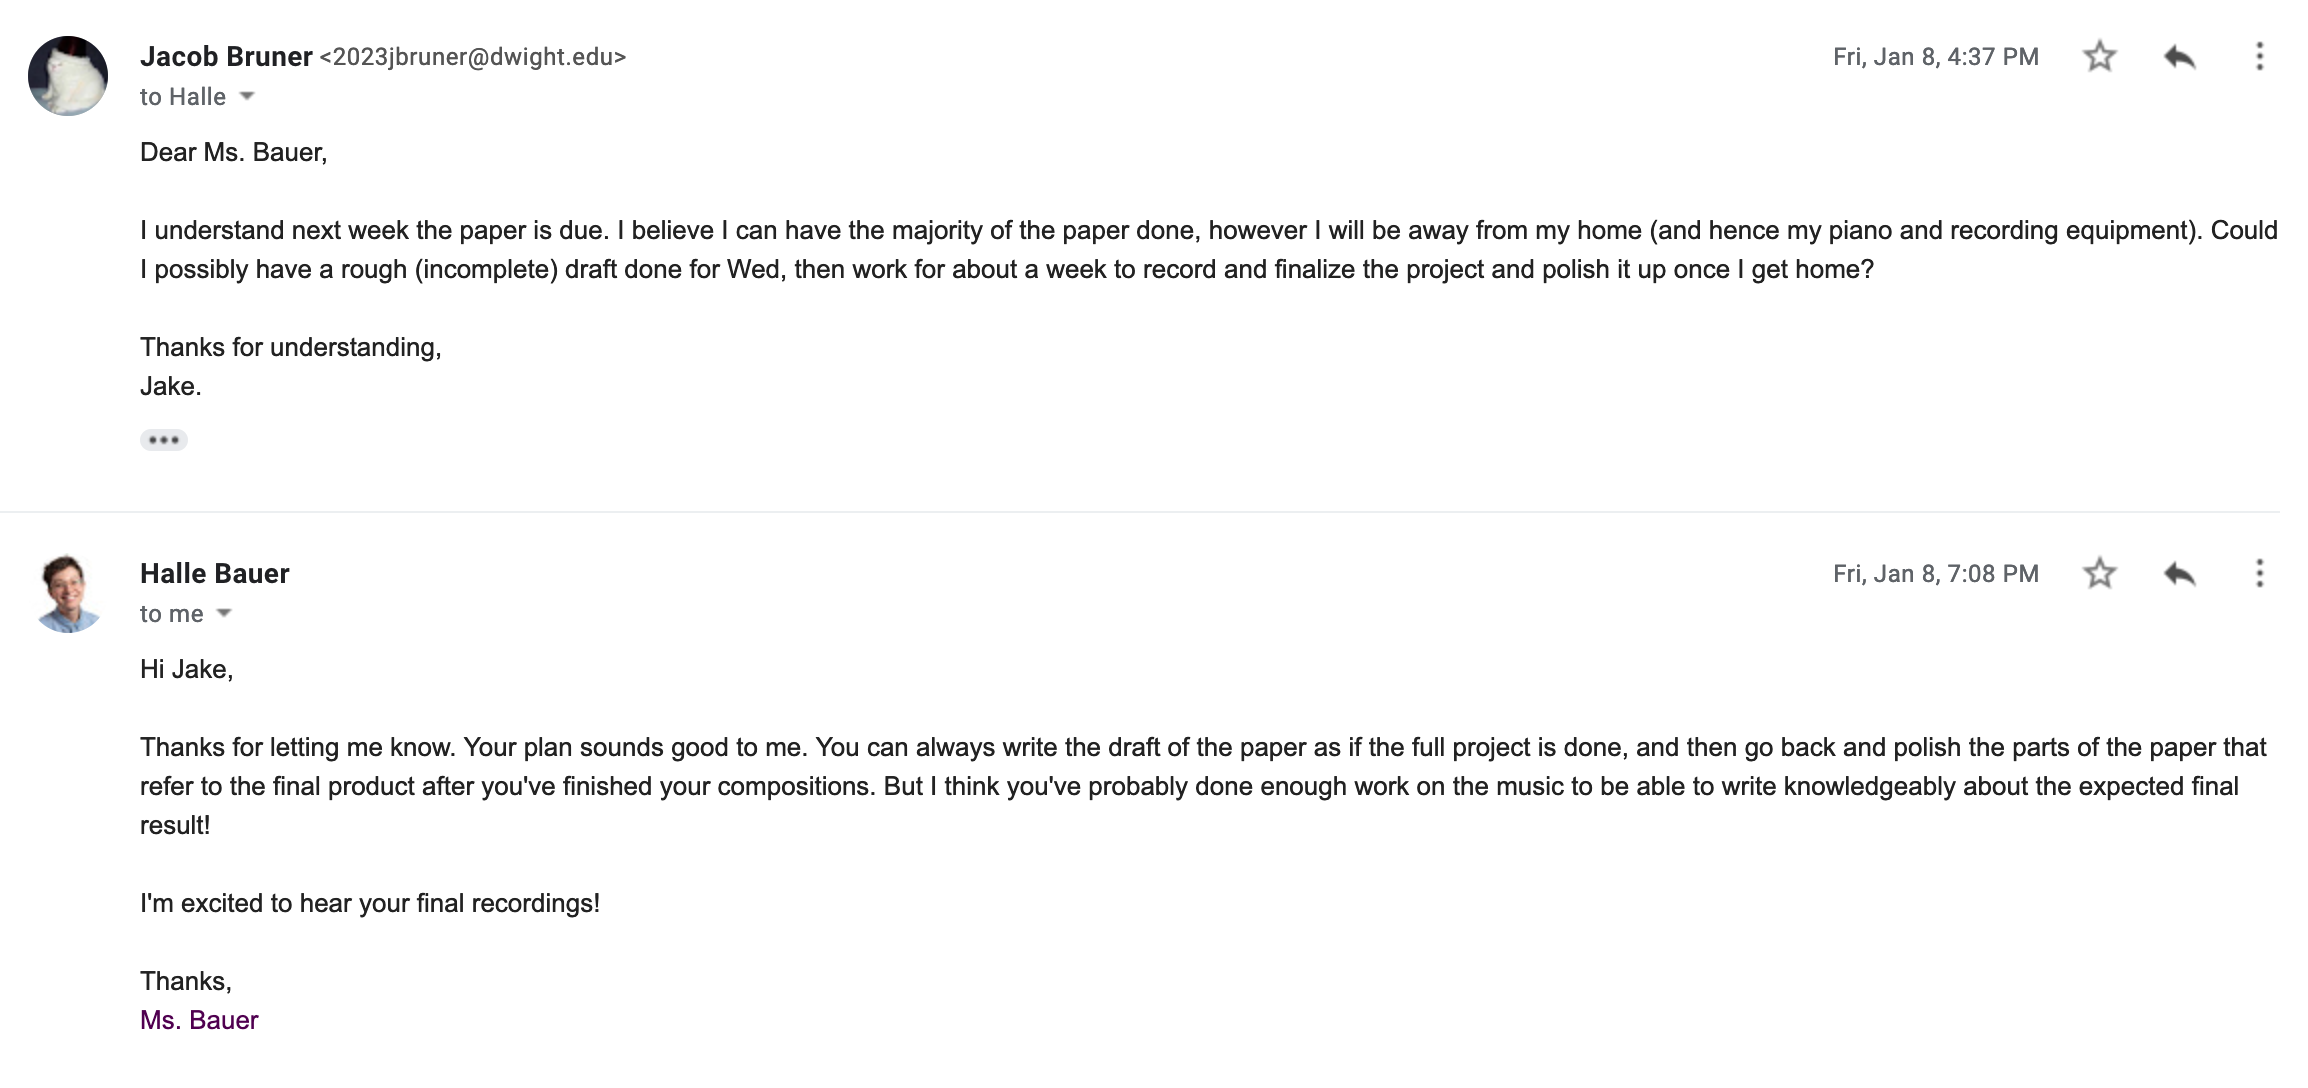
\includegraphics[scale=.43]{email3}

\end{center}

\newpage
\subsection*{Survey Form}
\begin{center}
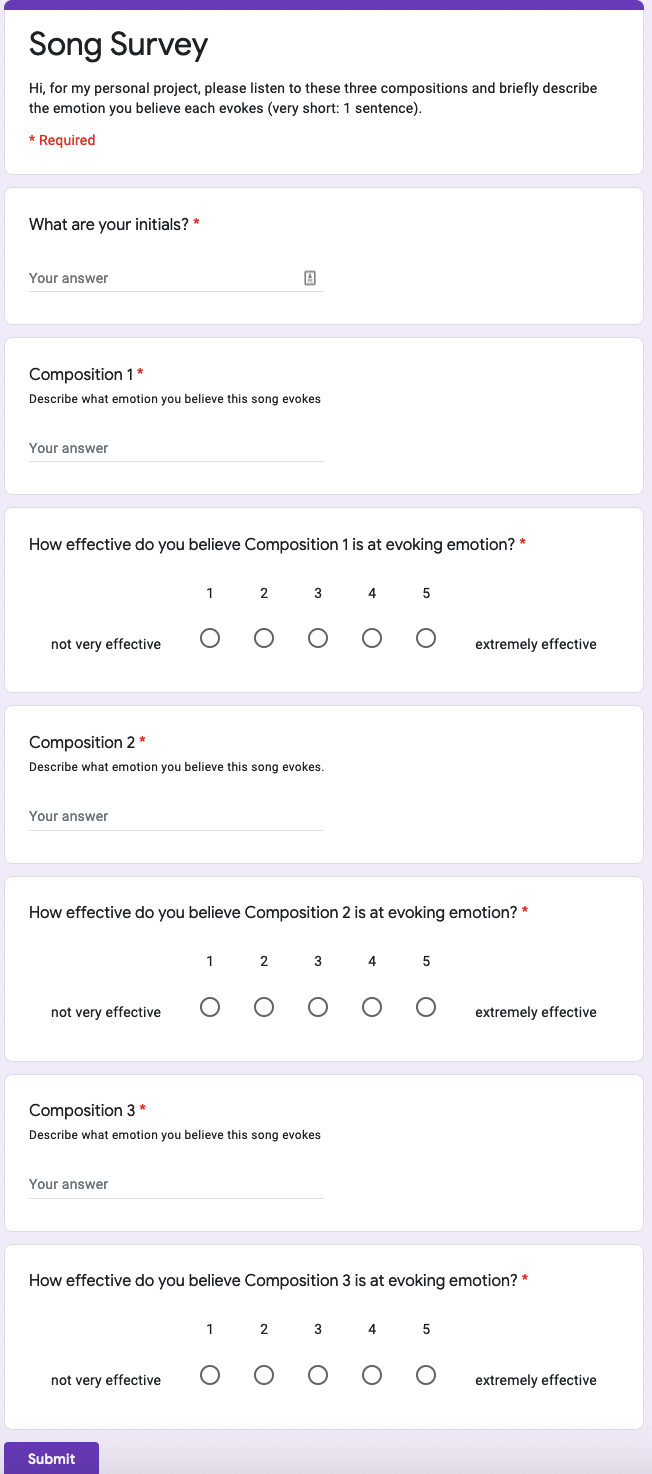
\includegraphics[scale=.8]{form}
\end{center}
\newpage
\subsection*{Survey Responses}
\begin{center}
\hspace*{-1.8cm}
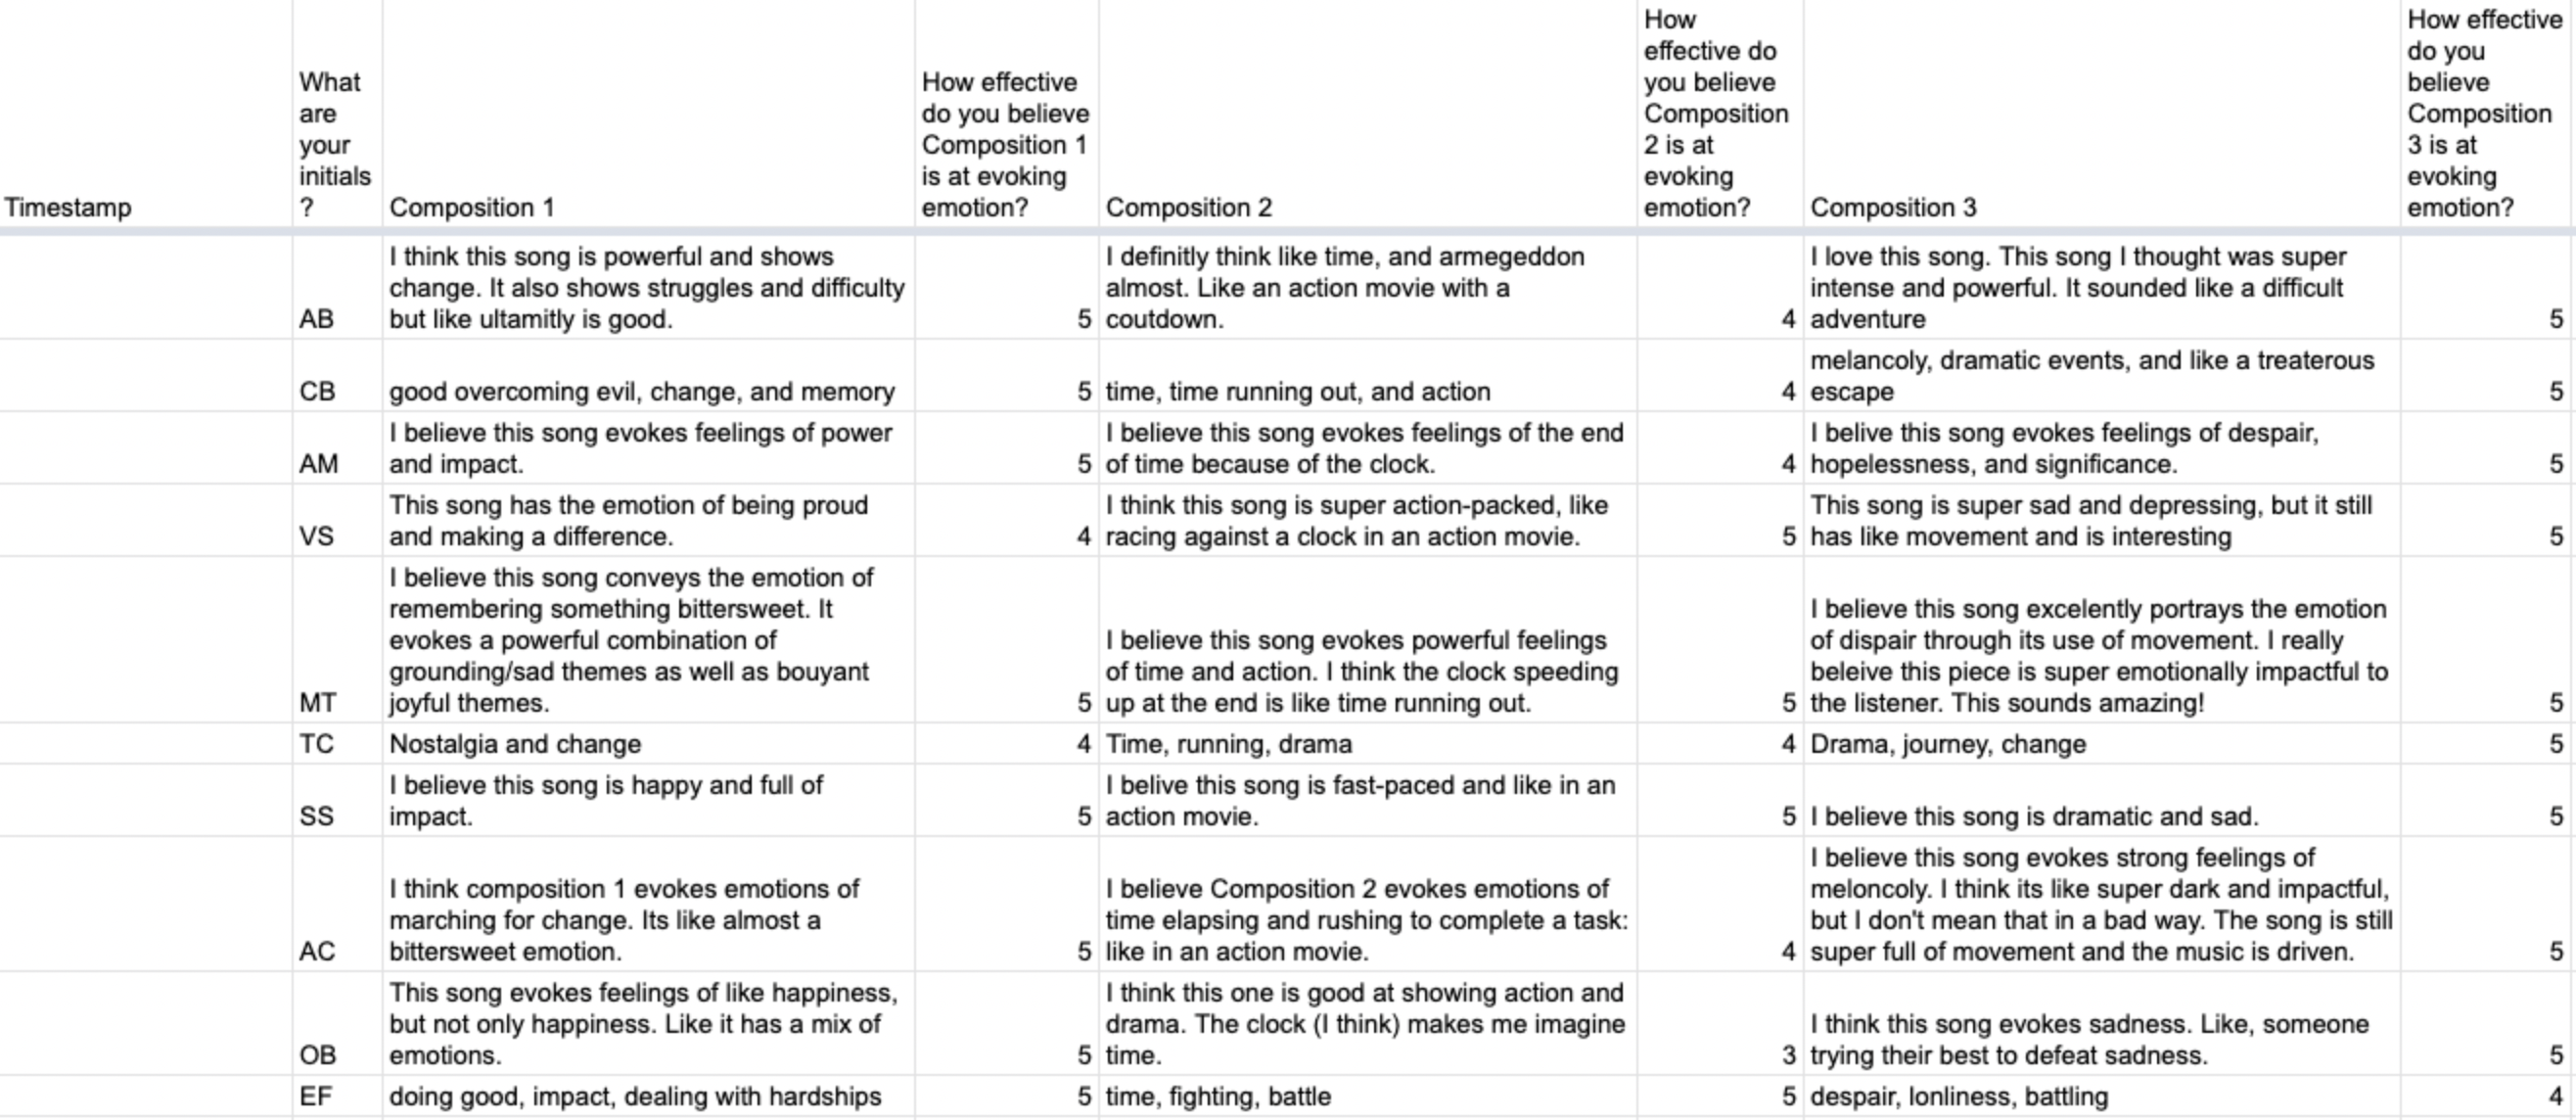
\includegraphics[scale=.4]{responses}
\end{center}

\newpage
\subsection*{Evidence of Music Planning}
\begin{center}
\hspace*{-1.5cm}
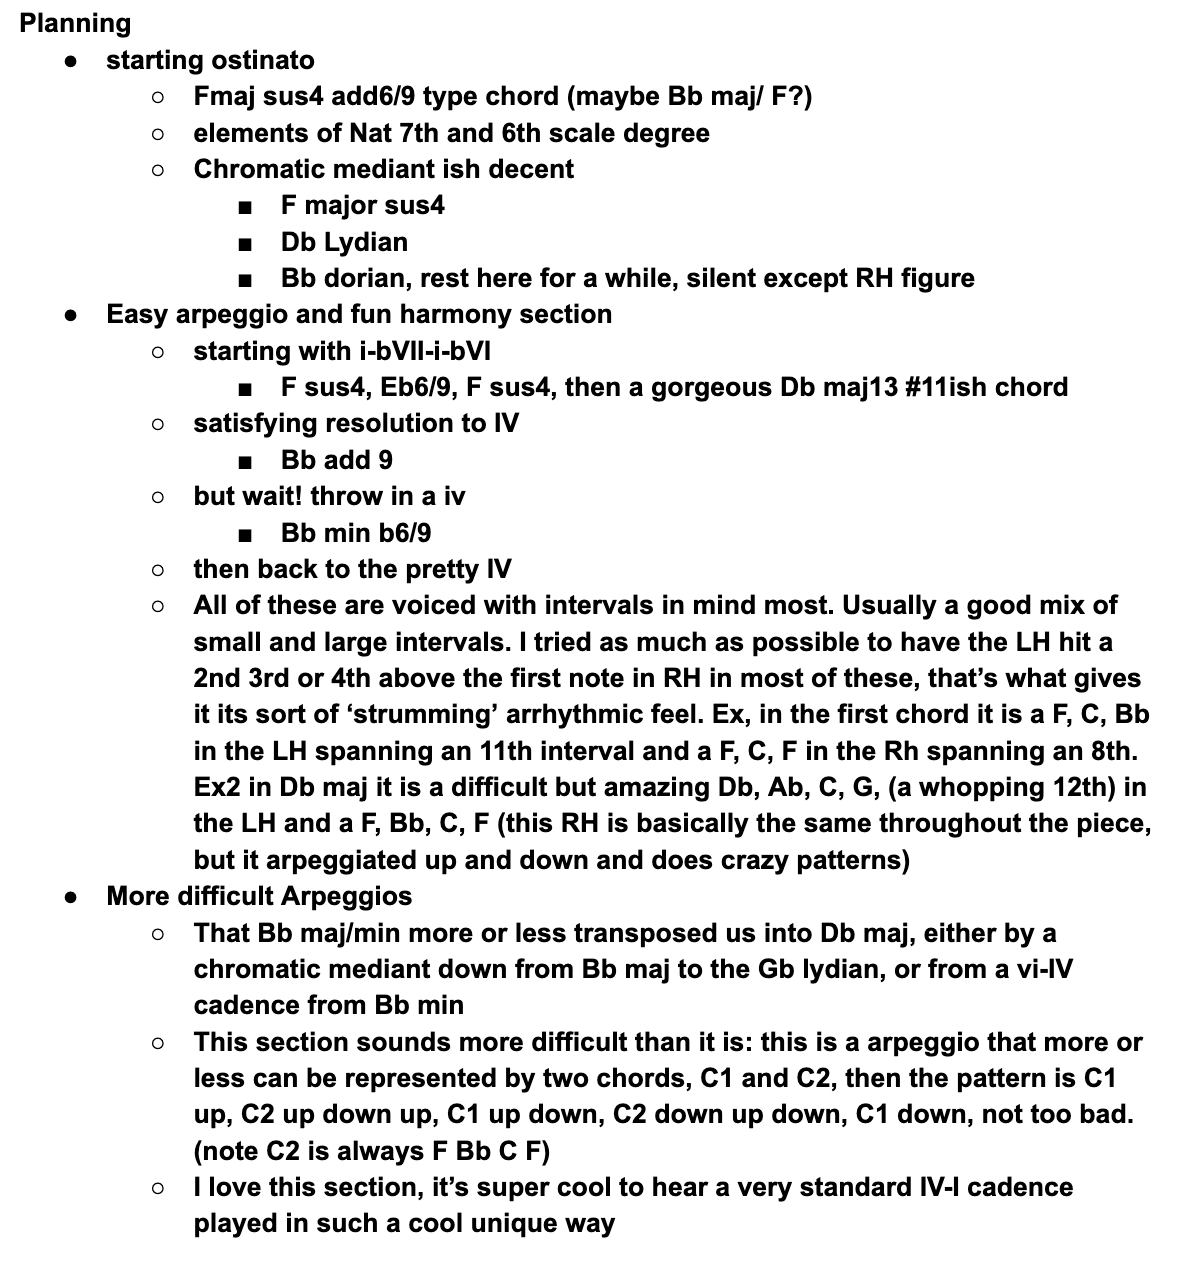
\includegraphics[scale=.85]{planning}
\end{center}

\newpage
\subsection*{Rubric of Criteria}
\begin{center}
\hspace*{-1.9cm}
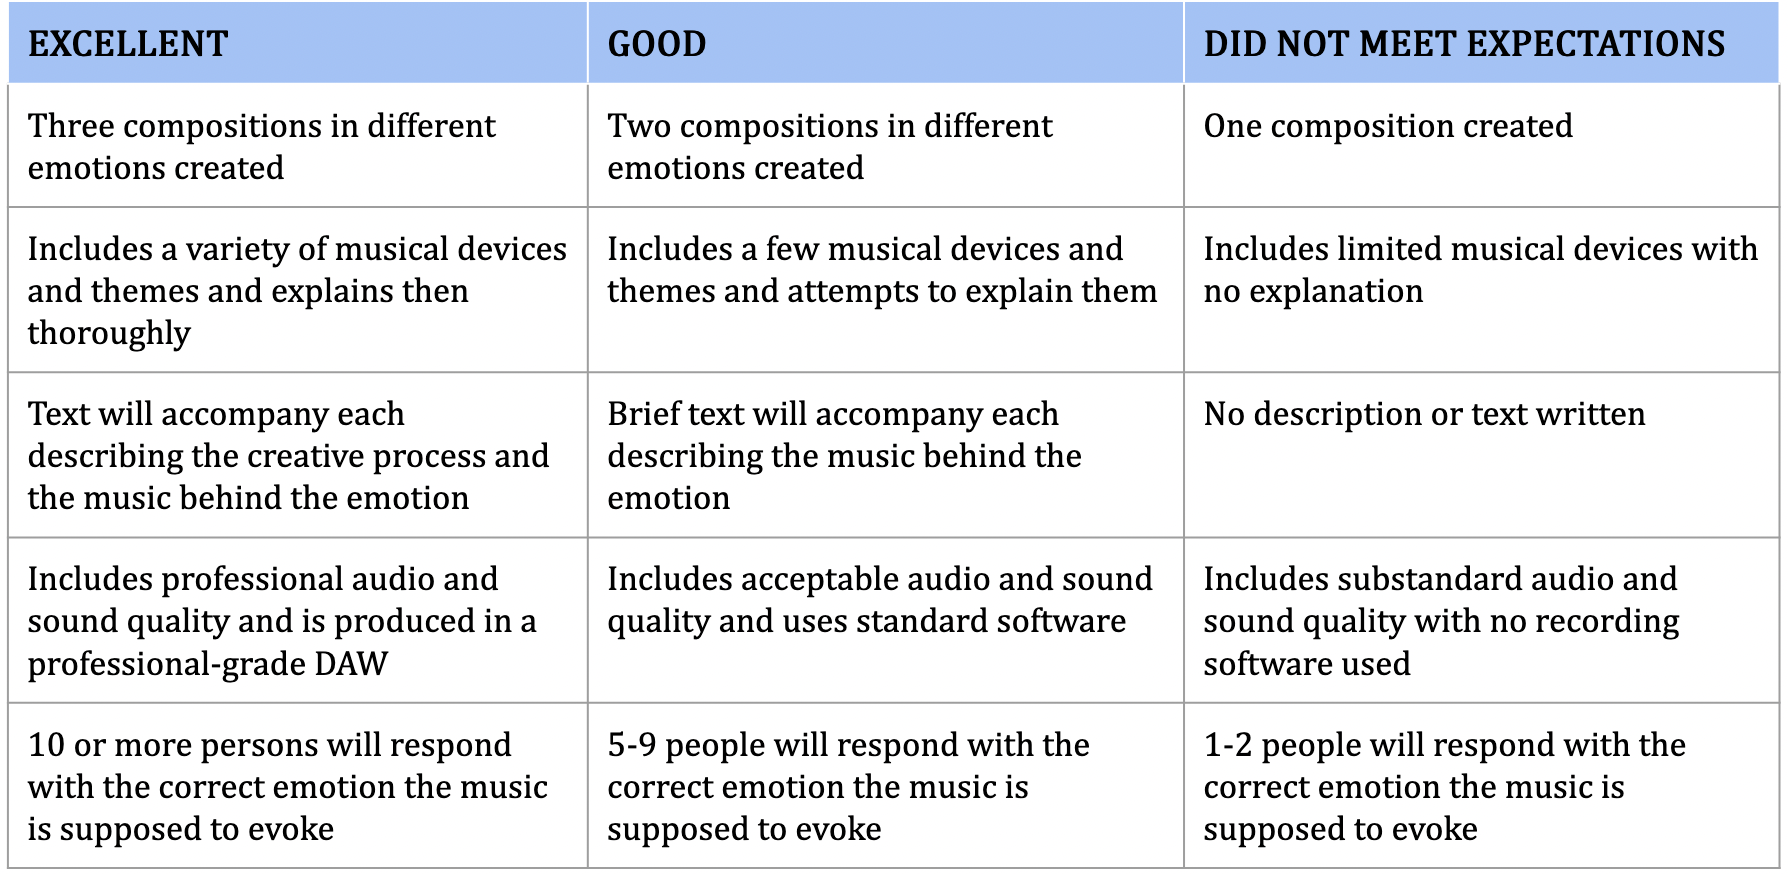
\includegraphics[scale=.6]{rubric}
\end{center}

\newpage
\subsection*{Self Assessment}
\begin{center}
\hspace*{-1.4cm}
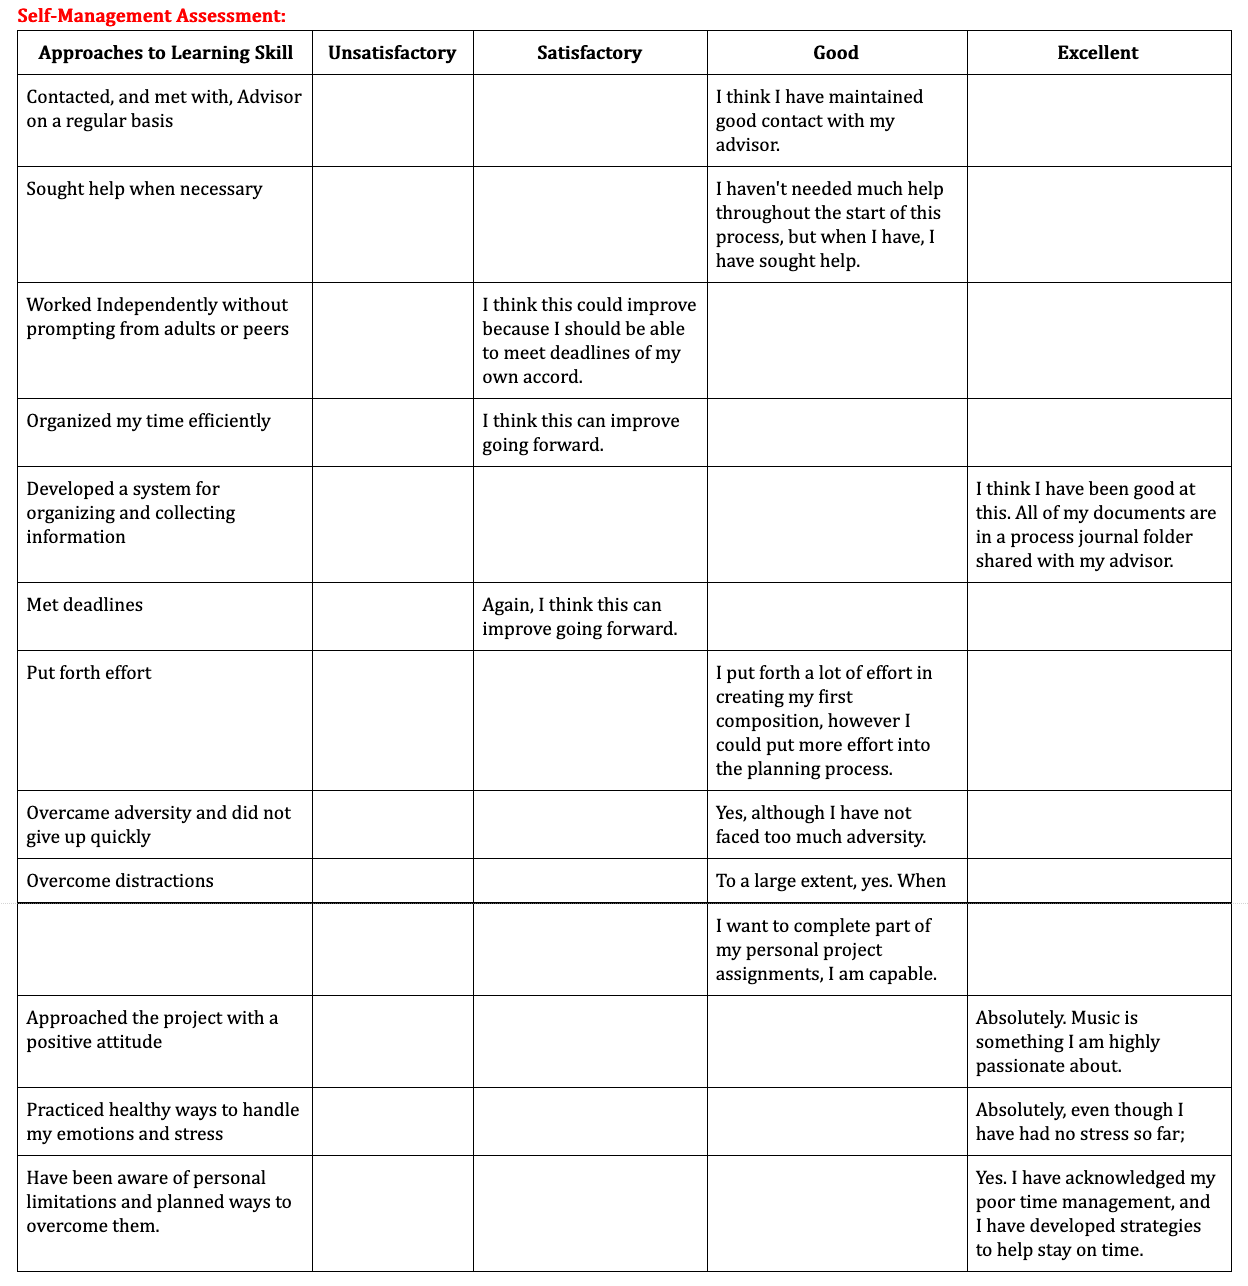
\includegraphics[scale=.8]{selfassess}
\end{center}
%-----------------------%
\newpage
\section{Bibliography}
\begin{center}
\hspace*{-1.5cm}
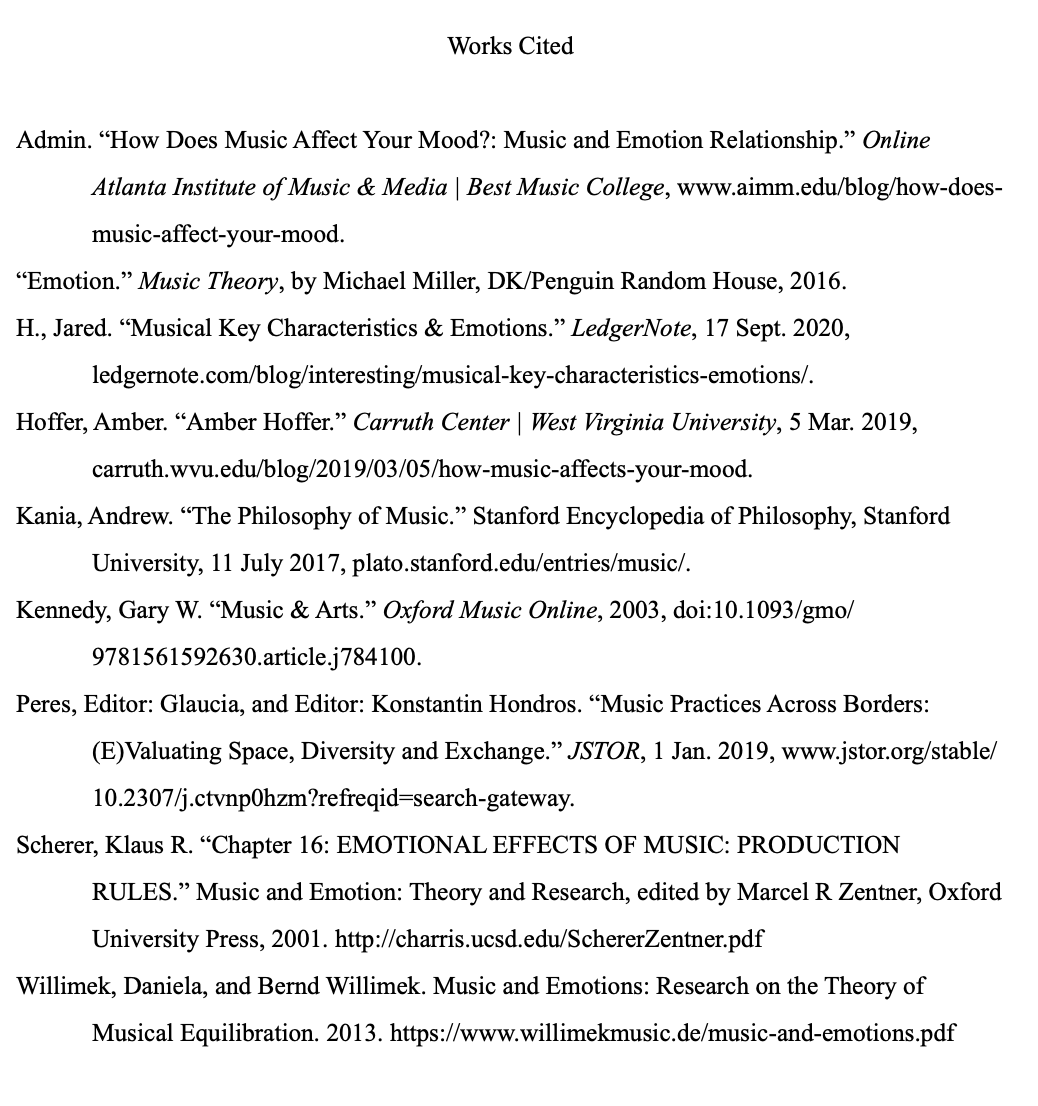
\includegraphics[scale=1]{citations}
\end{center}
\end{document}